\section{Additional Details on 2D Push-Pull Block Puzzles Proof}

This section provides some additional figures and description to help explain the proof of Theorem~\ref{thm:2DNPhard}.

Here we walk through the allowable transitions in the Set-Verify gadget and also address the potential Broken state in the Push-Pull construction which is not in the abstract gadget. In the Unset state, the $S_i \rightarrow S_o$ transition is the only possibility, changing the state to Set. In the Set state, the $S_o \rightarrow S_i$ transition is possible, changing the state back to Unset, as well as the $V_i \rightarrow V_o$ transition, which changes the state to Verified. Finally, from the Verified state, the only transitions possible are $V_o \rightarrow V_i$, changing the state back to Set, and $V_i \rightarrow V_o$, leaving the state as Verified. In the Broken state, the only possible transition is $S_o \rightarrow S_i$, changing the state to Unset. Any time we would enter the Broken state, we could instead enter the Set state, which allows strictly more transitions, and therefore will be strictly more helpful in reaching the goal. The Broken state is not helpful towards reaching the goal, so we will disregard its existence.

For the Set-Verify gadget in the Unset state, the $S_i$ entrance is the only one which allows the robot to move any blocks. From the $S_i$ entrance it can traverse to $S_o$, and it can also pull block $2$ down behind them. Doing so will allow a traversal from $V_i$ to $V_o$. To traverse back from $S_o$ to $S_i$, the robot must first traverse back from $V_o$ to $V_i$. Then, when the robot travels back from $S_o$ to $S_i$, it must push block $2$ back, ensuring the $V_i$ to $V_o$ traversal is impossible. Further, access to any sequence of entrances will not allow the robot to alter the system to allow traversals between the $V_i$ and $S_i$ entrances. 

\begin{figure}[!ht]
\begin{minipage}{.36\textwidth}
    \includegraphics[width=\textwidth]{NPClauseGadget}
    \caption{Clause gadget, $C_k$, with variables $x_a=1$, $x_b=0$, $x_c=0$.}
    \label{fig:NPClauseGadget}
\end{minipage}
\hspace{5mm}
\begin{minipage}{.57\textwidth}
  \centering
    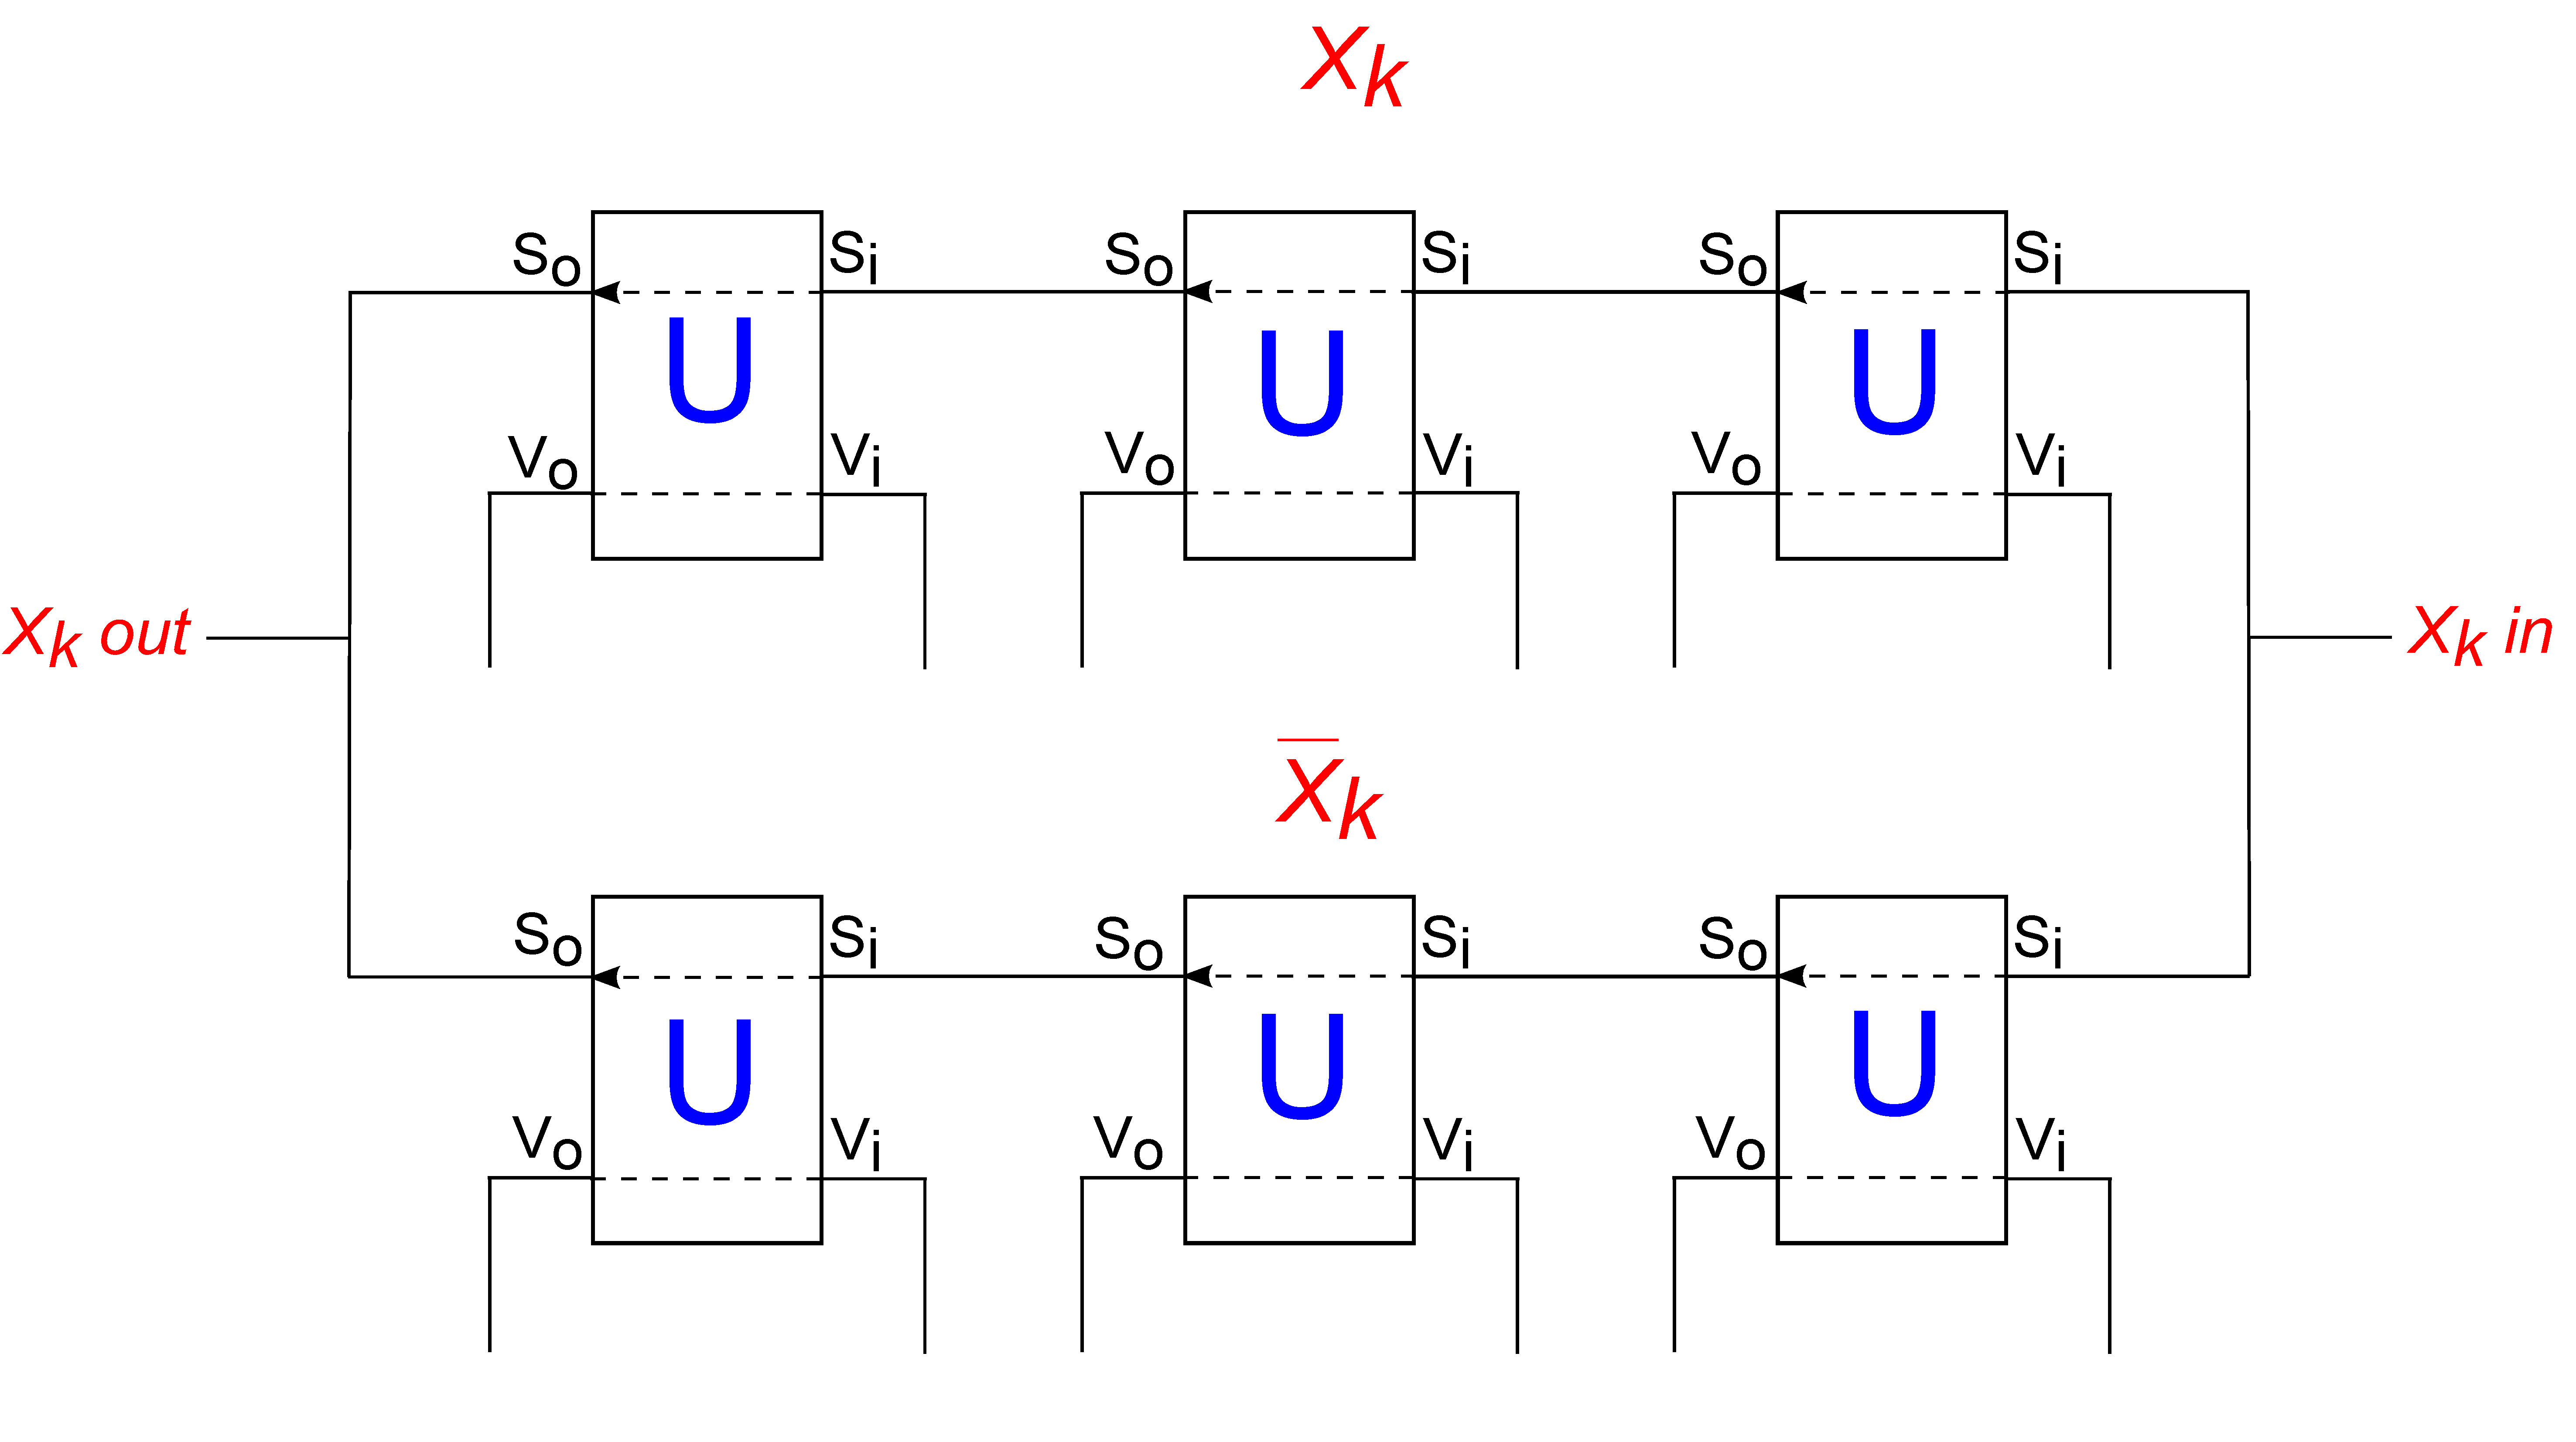
\includegraphics[width=.8\textwidth]{NPVariableGadget}
    \caption{A variable gadget representing $X_k$ occurring in six clauses, three of those times negated. The value of the variable has been set to true.}
    \label{fig:NPVariableGadget}
\end{minipage}
\end{figure}


\subsubsection{Crossover Gadgets}
\label{sec:NPCrossover}
In this section we build up the needed two use crossover gadget from a series of weaker types of crossover gadgets. One may wonder why we need crossover gadgets when Planar 3SAT is NP-complete. This only guarantees that connecting the vertices to their clauses by edges results in a planar graph, it does not ensure that we can navigate our robot between all of these gadgets in a planar manner or that our gadgets themselves are planar. The most obvious issue can be seen in the clause gadget (Figure~\ref{fig:NPClauseGadget}) where one of the Set Verify gadgets must lie between the other two hallways, but must also be accessible by its associated variable gadget.

\paragraph{Directed Destructive Crossover} This gadget, depicted in Figure~\ref{fig:DestructiveCrossover}, allows either a traversal from $a$ to $a'$ or $b$ to $b'$. Once a traversal has occurred, that path may be traversed in reverse, but the other is impassable unless the original traversal is undone.

First, observe that transitions are initially only possible via the $a$ and $b$ entrances, since the transitions possible through a Set-Verify in the Set state can be entered through $V_i$ and $S_o$, not $S_i$. Assume without loss of generality that the gadget is entered at $a$. This changes the state of the left Set-Verify to Verified. At this point, only the right $S_o$ and left $V_o$ transitions are passable. Taking the $V_o$ transition either reverts all changes to the original state, or leaves the left crossover in the Verified state, which allows strictly less future transition than the original state. Therefore, we will disregard that option. Taking the $S_o$ transition changes the right Set-Verify to Unset, and completes the crossover. At this point, the only possible transition is to undo the transition just made, from $a'$ back to $a$, restoring the original state. The gadget could be entered via $a$, but the robot would only be able to leave via $a$, possibly changing the state to Set. Both options result in the robot exiting out its original entrance, and allow the same or less future transitions, so we may disregard those options. Thus, the only transition possibilities are as stated above.

\begin{figure}[!ht]
  \centering
  \begin{subfigure}[b]{0.47\textwidth}
    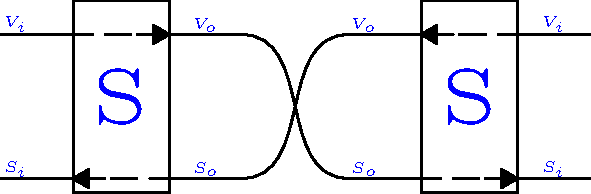
\includegraphics[width=\textwidth]{OneWayDestructiveCrossover}
    \caption{The directed destructive crossover constructed from two connected Set-Verify gadgets initialized in the set position.}
    \label{fig:DestructiveCrossover}
  \end{subfigure}
  \hfill
  \begin{subfigure}[b]{0.47\textwidth}
    \includegraphics[width=\textwidth]{InOrderCrossover}
    \caption{The in-order directed crossover constructed from two connected Set-Verify gadgets initialized in the verified and unset positions.}
    \label{fig:InOrderCrossover}
  \end{subfigure}
  \caption{Two types of crossover gadgets}
\end{figure}

%\begin{figure}[!ht]
%  \centering
%  \begin{subfigure}[b]{0.48\textwidth}
%    \includegraphics[width=\textwidth]{one_use_crossover}
%    \caption{The one use directed crossover is constructed from a directed destructive crossover and two in-order directed crossovers.}
%    \label{OneUseCrossover}
%  \end{subfigure}
%  \hfill
%  \begin{subfigure}[b]{0.43\textwidth}
%    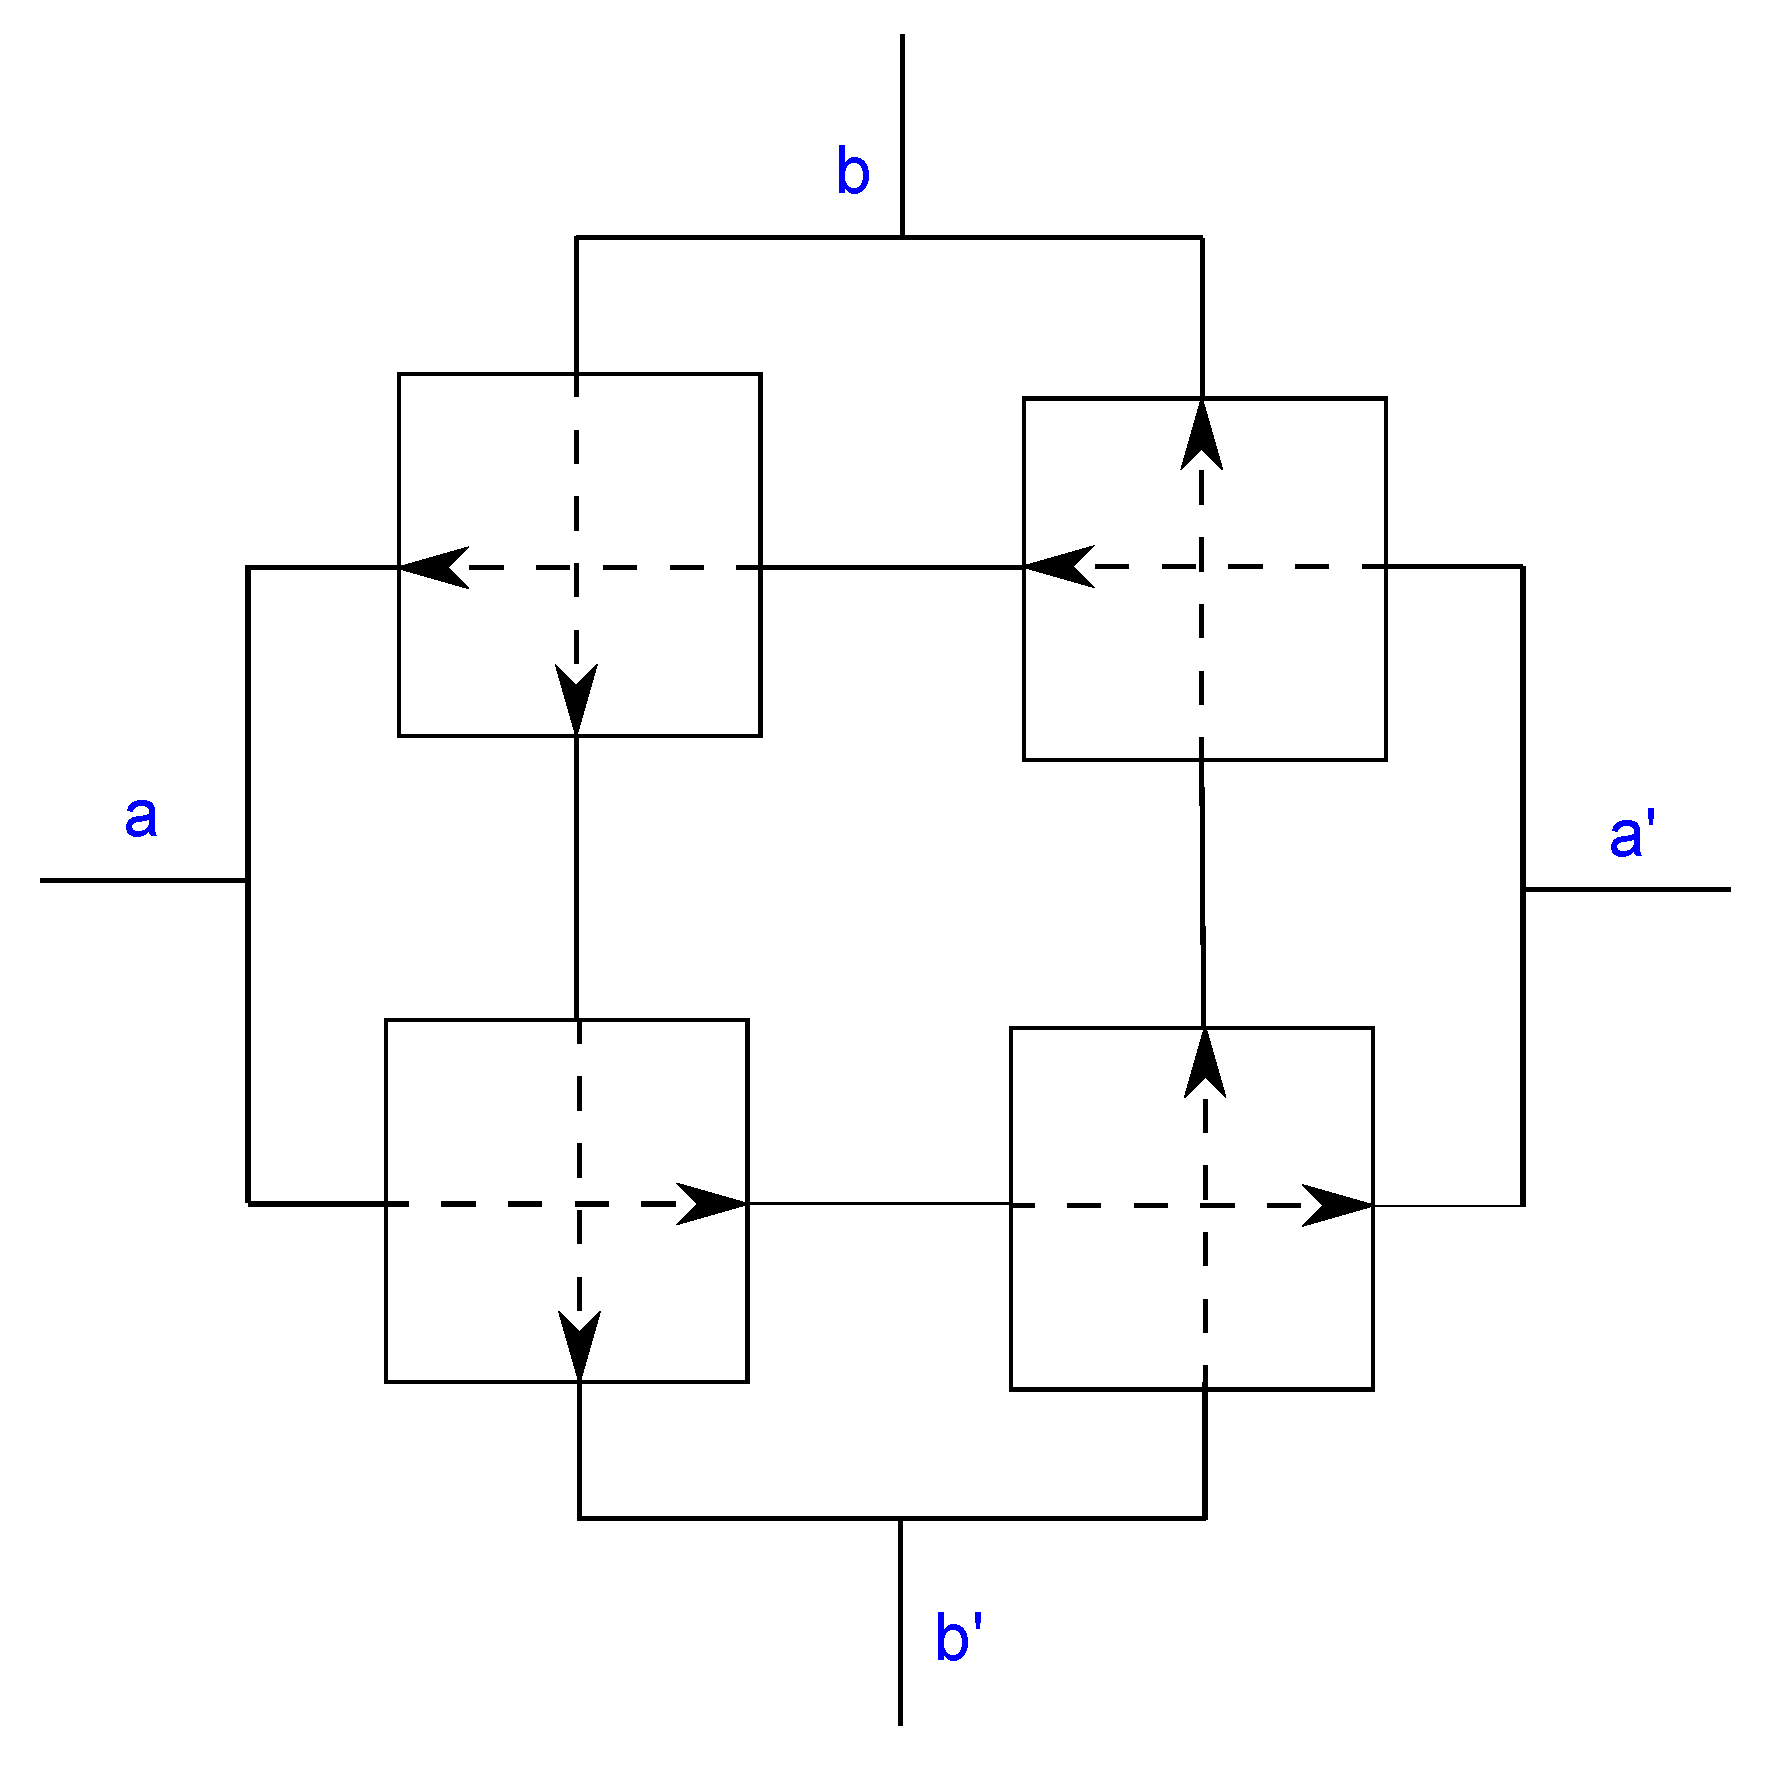
\includegraphics[width=\textwidth]{full_one_use_crossover}
%    \caption{A full one use crossover constructed from four directed one use crossovers.}
%    \label{full_one_use_crossover}
%  \end{subfigure}
%  \caption{Composite crossover gadgets}
%\end{figure}



\paragraph{In-order Directed Crossover} This gadget, depicted in Figure~\ref{fig:InOrderCrossover} allows a traversal from $a$ to $a'$, followed by a traversal from $b$ to $b'$. These traversals may also be reversed.

Initially, no entrance is passable except for $a$, since $V_o$ is passable only in the Verified state, and $S_o$ is
passable only in the Set state. Once the left $V_o \rightarrow V_i$ transition is made, the robot has 2 options.
It can either change the left Set-Verify gadget's state to Set, or leave it as Verified. In either case, the $S_i$
entrance on that toggle is impassable, since a $S_i$ entrance may only be traversed in the Unset state. The
only transition possible on the right crossover is $S_i \rightarrow S_o$, changing the state from Unset to Set.
This completes the first crossing.

Now, there are at most 2 transitions possible: from $a'$ back to $a$, undoing the whole process, or entering at $b$. Note that entering at $b$ is only possible if the left Set-Verify is in the Set state, so let us assume that state change occurred. In that case, the left $S_o \rightarrow S_i$ transition may be performed, changing the left Set-Verify's state to Unset. At that point, the only possible transitions are back to $b$, or through the right Set-Verify's
$V_i \rightarrow V_o$ transition, completing the second crossover.

\begin{wrapfigure}{hr}{0.45\textwidth}
\vspace{-5mm}
  \centering
    \includegraphics[width=.5\textwidth]{one_use_crossover}
    \caption{The two use directed crossover is constructed from a directed destructive crossover and two in-order directed crossovers.}
    \label{fig:OneUseCrossover}
    \vspace{-7mm}
\end{wrapfigure}

If the left Set-Verify was left in the Verify state, strictly less future transitions are possible compared to the case where it was changed into the set state, so we may disregard that possibility.


\paragraph{Two Use Directed Crossover} 
The Two Use Directed Crossover, depicted in Figure~\ref{fig:OneUseCrossover}, is the gadget needed for our proof. It allows a traversal from $a$ to $a'$ followed by a traversal from $b$ to $b'$, or from $b$ to $b'$ and then $a$ to $a'$. These transitions may also be reversed.

It is constructed out of an In-order Directed Crossover gadget and a Destructive Directed Crossover, as shown in Figure~\ref{fig:OneUseCrossover}. The $a$ to $a'$ traversal is initially passable, and goes through both gadgets,
blocking the destructive crossover but leaving the in-order crossover open for the $b$ to $b'$ traversal. If the $a$ to $a'$ traversal does not occur, the $b$ to $b'$ traversal is possible via the destructive crossover.


%\begin{wrapfigure}{hr}{0.45\textwidth}
%\vspace{-5mm}
%  \centering
%%  \begin{figure}[t]
%%    \centering
%    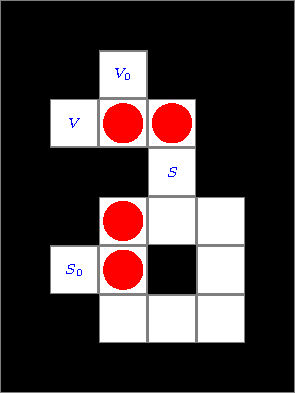
\includegraphics[width=.4\textwidth]{SetVerify3D}
%    \caption{A Set-Verify gadget in 3D where the entrances and exits extend upward, notated by the diagonal arrows. This gadget is in the unset state.}
%    \label{fig:3DSetVerify}
%    \vspace{-12mm}
%\end{wrapfigure}


Because of the behavior of the constituent crossovers which make up this gadget, no transition from $a$ to $b$ $a$ to $b'$, etc. is possible. The crossover permits reversal of each of the transitions described, but the crossings can only be reversed in queue order (last in, first out).
%
\paragraph{Two Use Crossover} 
Four Directed Crossovers can be combined, as shown below, to create a crossover that can be traversed in any direction \cite{Push100}. This is not necessary for our proof but is shown for general interest. Unfortunately, the inability to go through this gadget multiple times in the same direction without first going back through means it likely isn't sufficient for PSPACE-completeness. 

\section{3D Push-Pull is NP-hard}
\label{3DNPhard}
In this section we prove that 3D Push-$k$ Pull-$l$ with fixed blocks is NP-hard, for all positive $k$ and $l$. All of the hard work was done in Section~\ref{2DNPhard}. Here we will simply show how we can use the additional dimension to tweak the previous gadgets to build them without thin walls. We reduce from 3SAT, constructing our variables from chains of 3D Set-Verify gadgets, and our clauses from the verify side of the corresponding 3D Set-Verify gadget.

\begin{theorem}
3D Push-$k$ Pull-$l$ with fixed blocks is NP-hard, for all positive $k$ and $l$.
\end{theorem}
\begin{proof}
We follow the proof of Theorem~\ref{thm:2DNPhard} using a modified Set-Verify gadget, shown in Figure~\ref{fig:3DSetVerify}.  It can be easily checked that this has the same properties as the Set-Verify given in Section~\ref{sec:SetVerifyGadgets}. The cyclic ordering of the entrances in the 3D Set-Verify is different from that of the 2D Set-Verify, however this is not important as we no longer need to construct crossovers. Also, this construction does not use thin-walls. While this was critical in the prior construction due to the need for closely packed turns, the additional dimension allows enough freedom to keep separate hallways from being adjacent to each other. With a functional Set-Verify gadget, the remaining constructions of variables and clauses proceeded as in Section \ref{sec:2DPushPull3SAT}. No crossover gadgets are needed since we are working in 3D. Finally, we note that all blocks are in hallways of length at most 3, thus the gadgets still function as described for any positive push and pull values.

\begin{figure}{hr}
\vspace{-5mm}
  \centering
%  \begin{figure}[t]
%    \centering
    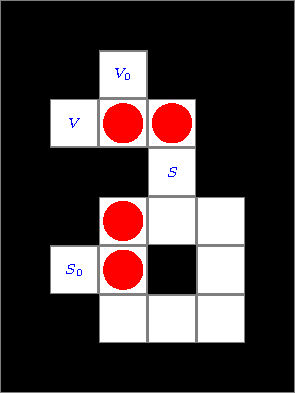
\includegraphics[width=.4\textwidth]{SetVerify3D}
    \caption{A Set-Verify gadget in 3D where the entrances and exits extend upward, notated by the diagonal arrows. This gadget is in the unset state.}
    \label{fig:3DSetVerify}
    \vspace{-12mm}
\end{figure}

\section{Additional Details on PSPACE-completeness Proof}

This section provides some additional figures and description to help explain the proof of Theorem~\ref{thm:3dPSPACE-complete}.

\begin{figure}[!ht]
  \centering
  \begin{subfigure}[t]{.45\textwidth}
    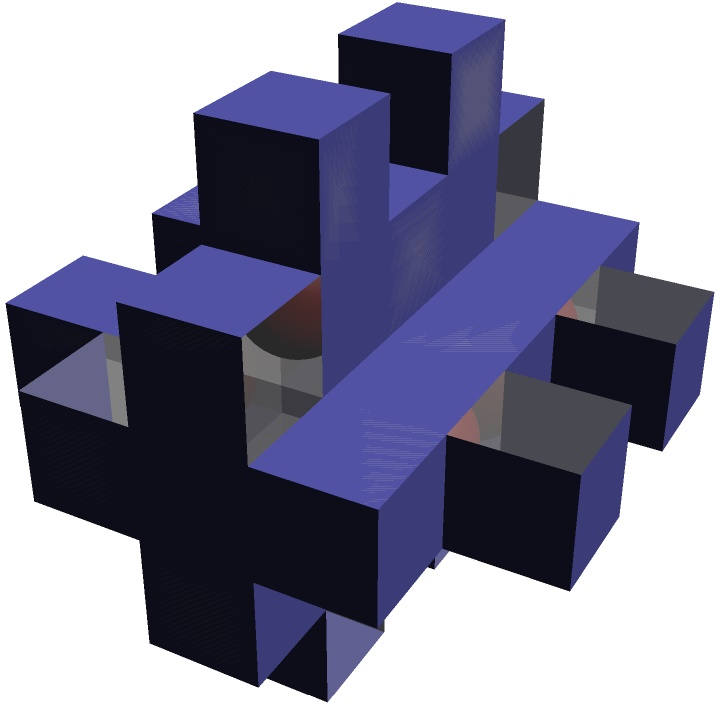
\includegraphics[width=\linewidth]{4ToggleNoConnections.jpg}
    \caption{Diagram of a 4-toggle showing impassible surfaces.}
    \label{fig:4Toggle3D}
%    \includemedia[width=0.3\linewidth,]{}{4Toggle.pdf}
  \end{subfigure}
  \hfill
  \begin{subfigure}[t]{.45\textwidth}
    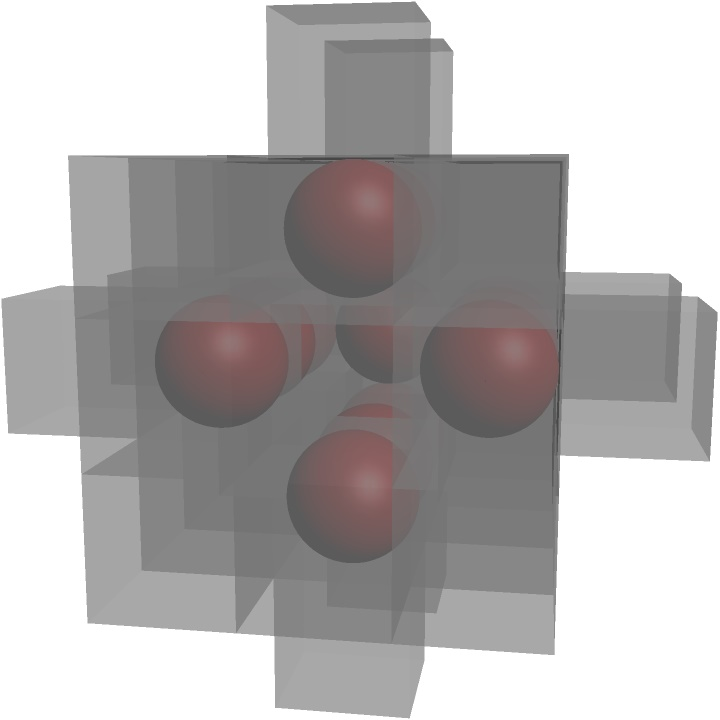
\includegraphics[width=\linewidth]{4ToggleBasic.jpg}
    \caption{Diagram of the internals of a 4-toggle.}
    \label{fig:4Toggle3DBasic}
  \end{subfigure}
  \caption{3D diagrams of 4-toggles. Red spheres are blocks and blue surfaces are impassable.}
\end{figure}

\begin{wrapfigure}{tr}{0.45\textwidth}
\vspace{-5mm}
  \centering
%  \begin{subfigure}[t]{0.45\textwidth}
%    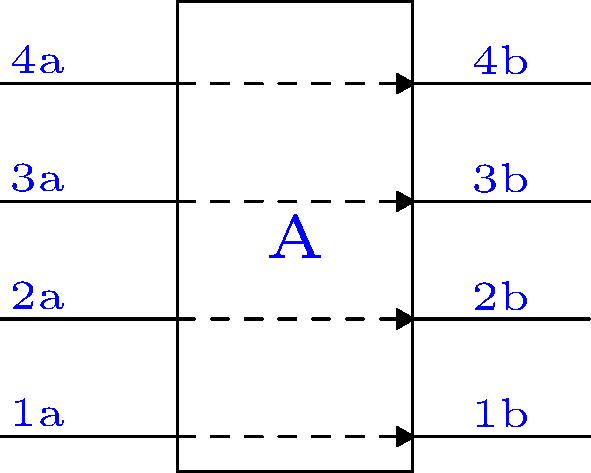
\includegraphics[width=\textwidth]{Abstract4ToggleA}
%    \caption{Representation of a 4-toggle in state $A$. }
%    \label{fig:4Toggle3D}
%  \end{subfigure}
%  \hfill
%  \begin{subfigure}[t]{0.45\textwidth}
    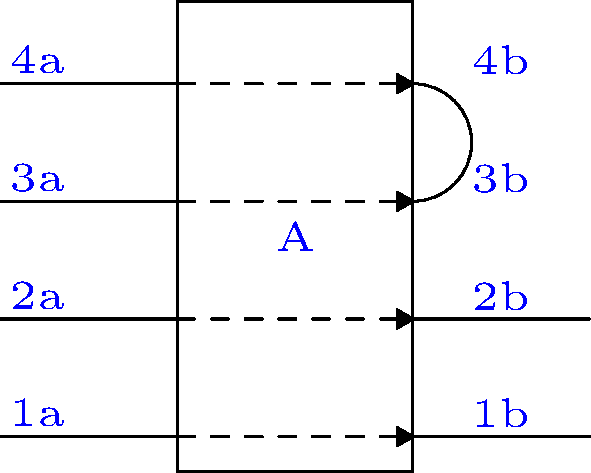
\includegraphics[width=.4\textwidth]{LockB}
    \caption{Diagram of a lock. The $3a$ to $4a$ traversal is only possible in state $A$ and returns the toggle to state $A$.}
    \label{fig:LockA}
%  \end{subfigure}
%  \caption{}
\vspace{-7mm}
\end{wrapfigure}

\begin{figure}[h!]
\centering
    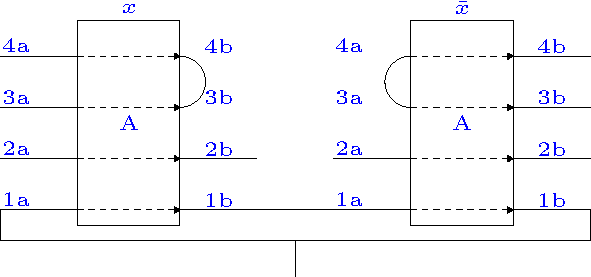
\includegraphics[width=0.8\textwidth]{existentialGadget}
    \caption{An existential gadget.} % is simply a 2-toggle and many locks with a lock for each literal corresponding to the appropriate variable that appears in the formula.
    \label{fig:Existential}
\end{figure}

\subsubsection{Binary Counter}
\label{sec:BinaryCounter}
Universal quantifiers must iterate through all possible combinations of values that they can take. In this section we construct a gadget that runs though all the states of its subcomponents as the robot progresses through the gadget. This construction will serve as the base for our universal quantifiers.

\begin{figure}[h!]
\centering
    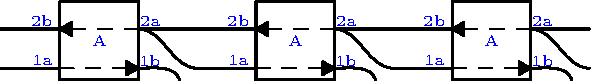
\includegraphics[width=.9\textwidth]{BinaryCounter}
    \caption{The central portion of a three bit binary counter made from 2-toggles.}
    \label{fig:BinaryCounter}
\end{figure}
  
A binary counter has a fixed number of internal bits.
Whenever the binary counter is traversed in the forwards direction, the binary number
formed by the internal bits increases by one and the robot leaves via one of the exits.
If the binary counter is traversed in the reverse direction, the internal value is reduced by
one. If the binary counter is partially traversed, but then the robot leaves via its initial entrance,
the internal value does not change.

%The binary counter is implemented as a series of 2-toggles, as shown in Figure~\ref{fig:BinaryCounter}.
%The entrance pathway is connected to the 2-toggle's $1A$ and $2B$ entrances. The $1B$ exit from the 2-toggle
%will exit from the entire binary counter. The $2A$ exit will continue on to the next 2-toggle,
%attaching to that toggle's $1A$ and $2B$ entrances. This will continue for every toggle down the line, except
%that the last toggle's $2A$ exit signals an overflow and exits from the counter.

The binary counter is implemented as a series of 2-toggles, as shown in Figure~\ref{fig:BinaryCounter}.
To see that this produces the desired effect, identify a toggle in state $A$ as a $0$ bit, and a toggle in state
$B$ as a $1$ bit. Let the entrance toggle's bit be the least significant bit, and the final toggle be the
most significant. When the robot enters the binary counter in the forwards direction, it will flip
the state of every toggle it passes through. When it enters a toggle that is initially in state $B$, and thus whose
bit is $1$, it will flip the state/bit and proceed to the next toggle, via the $2B - 2A$ pathway. When it
encounters a toggle that is initially in state $A$ / bit $0$, it will flip the state/bit and exit via the $1A - 1B$
pathway. Thus, the overall effect on the bits of the binary counter is to change a sequence of bits ending at the
least significant bit from $01\ldots11$ to $10\ldots00$, where the entrance is at the right.
This has the effect of increasing the value of the binary counter by one.
We will not examine the reverse transitions or rigorously complete the binary counter here, 
as we do not use it directly in the final construction. 

%As before, in the unset state the only possible traversal is $S_i$ to $S_0$. This traversal allows the top right bock to be pulled down, moving the gadget into the set state. From here the $V$ to $V_0$ traversal is possible, as well as going back through the $S_0$ to $S$ pathway. However, the $S$ to $S_0$ traversal is not possible.

%Variables are composed of hallways of 3D Set-Verify gadgets connected $S_0$ to $S$, one for each clause in which the variable appears, as in Figure~\ref{fig:NPVariableGadget}. Clauses are composed of three 3D Set-Verify gadgets connected in parallel as in Figure~\ref{fig:NPClauseGadget}. The details of these constructions follow those in Section~\ref{sec:2DPushPull3SAT} This completes the reduction from 3SAT. In addition, we note that all blocks are in hallways of length at most 3, thus the gadgets still function as described for any positive push and pull values.

\subsubsection{Analysis of the Quantifier Chain}
\label{sec:AnalysisQuantifierChain}

A quantifier chain is implemented much like a binary counter (Section~\ref{sec:BinaryCounter}), with some additions. Every universal variable will be represented by a 2-toggle and many locks, where individual locks will serve as a literal. The 2-toggles are hooked up in the same manner as the 2-toggles in a binary counter gadget. This forces the 2-toggle and many locks gadgets to be set to the corresponding values in the simulated binary counter.

Traversing  the quantifier chain in the reverse direction is only possible if the robot enters
via the lowest order universal toggle whose setting is $1$. The traversal will go back one setting in the
sequence of possible settings of the universal variables, and allow the robot to set all existential variables
corresponding to altered universal variables arbitrarily. No other existential variables can be changed.

There is also a special exit, the overflow exit, which can only be
reached after all of the universal variable settings have been traversed. This is the goal location for the robot.

The next addition is the existential variables, which consist of existential gadgets placed just after the $2A$
exits of each universal variable,
and just before the $1A$ and $2B$ entrances of the next universal variable, as shown
in Figure~\ref{fig:QuantifierChain}.

One portion of the apparatus which has not been analyzed thus far is the potential for the robot to re-enter the chain of existentials
via a different exit pathway than the one just exited. This would be problematic if the robot re-entered via a universal gadget it had not just exited,
both because the robot should not be able to take any action other than reversing its prior progress, 
decrementing the binary counter/universal quantifiers. Problems would also arise if the robot got access to any existential quantifiers 
it did not just traverse.

After a traversal, the universal quantifiers have the settings $\ldots??10\ldots00$, where the lowest significance $1$ is 
on the pathway just exited.
To prevent the robot from re-entering via any pathway other than the one just exited, we add a series of locks to each exit that are only passable
if all lower-significance universal toggles are in state $0$, as shown in Figure~\ref{fig:QuantifierChain}.
This does not impede the exit that the robot uses initially, since all
lower-significance universal toggles are indeed $0$. These locks do prevent re-entry into any higher-significance universal toggles, since the
lock corresponding to the lowest-significance $1$ will be closed. The robot cannot re-enter via any toggle that is in state $0$,
due to the arrangement of the toggle pathways. Thus, the unique re-enterable pathway is the lowest-significance toggle in state $1$, as desired.

\end{proof}




